\section{Бетатрон в $\delta_{\mathrm{eq}}$}
\textbf{Вопрос.} На сколько сдвигается среднее $\delta$, если к той же частице добавить бетатрон?

$A_x=\vAxten$~мм, полость включена, $N=\vNbeta$ оборотов. Две формулы: без $\Lambda$ и с $\Lambda=-(2\pi/C)J_x\xi_x$.

\begin{figure}[H]\centering
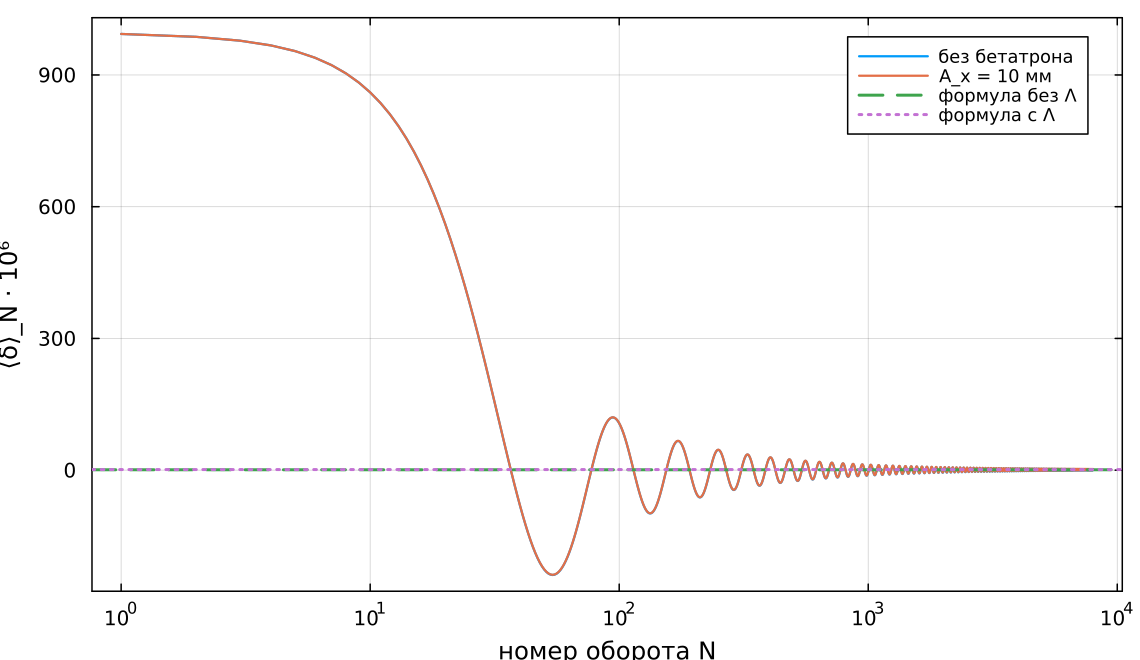
\includegraphics[width=0.92\textwidth]{figs/fig_06_lambda.png}
\caption{Формула без $\Lambda$: $\vMoneNoLam$. С $\Lambda$: $\vMoneLam$, сдвиг $\vLamShift$. Среднее интегратора $\vMeanLam$ (до формулы с $\Lambda$: $\vDiffLamMean$). M2: $\vMtwoLam$.}
\end{figure}

\textbf{Вывод.} Бетатрон сдвигает уровень на $\vLamShift$. Среднее садится на формулу с $\Lambda$, а не на формулу без него.
